\section{Footstep Evaluation Network}

\begin{todo}
  purpose
\end{todo}

%%%%%%%%%%%%%%%%%%%%%%%%%%%%%%%%%%%%%%%%%%%%%%%%%%%%%%%%%%%%%%%%%%%%%%%%%%%%%%%%
\subsection{Architecture}

The footstep evaluation neural network architecture, shown in
\autoref{fig:diagram-contactnet-architecture}, accomplishes a similar
task to ContactNet \cite{bratta_contactnet_2024}. It takes in robot state
information and ranks each of the possible footstep
positions. The architecture consists of a feedforward neural
network that first maps the input through two fully connected layers
of 64 units each, with ReLU activations. The resulting 64-dimensional
feature vector is reshaped into an 8x8 spatial representation and
processed by a convolutional layer with two output channels, a
3x3 kernel, with stride 1, and padding 1, followed by a ReLU
nonlinearity. The output is flattened and passed to a final
fully connected layer before being reshaped into a 5x5 grid.

\begin{figure}
  \centering
  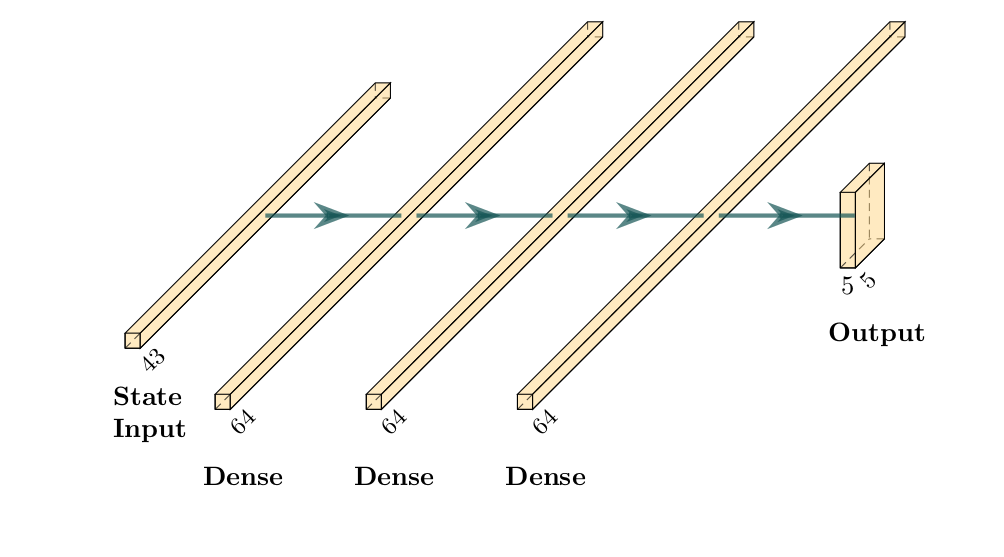
\includegraphics[width=0.5\linewidth]{images/diagrams/contact-network-architecture.png}
  \caption{Footstep evaluation neural network architecture.}
  \label{fig:diagram-contactnet-architecture}
\end{figure}

%%%%%%%%%%%%%%%%%%%%%%%%%%%%%%%%%%%%%%%%%%%%%%%%%%%%%%%%%%%%%%%%%%%%%%%%%%%%%%%%
\subsection{Training}

\begin{todo}
  Explain how we gathered the training data
\end{todo}

The factors that make up the footstep cost maps in the training data
are shown in \autoref{fig:costmap-composition-elements}, while the
combined cost map is shown in \autoref{fig:costmap-composition-combined}.
The most significant factors are the support polygon stability,
measured as the distance from the COM to the nearest edge of the
support polygon (\textit{inscribed\_circle\_radius}), and the
distance from the nominal foot position
(\textit{foot\_hip\_distance}). Other factors make up a small, but
still important part of the cost map. These include
\textit{lin\_vel\_z\_l2} which penalizes high vertical velocity,
\textit{ang\_vel\_xy\_l2} which penalizes high angular velocity in
the horizontal plane, \textit{joint\_torques\_l2} which penalizes
high joint torques, \textit{joint\_acc\_l2} which penalizes high
joint accelerations, and \textit{control\_error}, which penalizes
errors in the swing duration between the requested and actual values.
Some of these factors are balanced to have a lower spread, mitigating
factors that consistently prefer one leg over another.

\begin{figure}
  \centering
  \begin{subfigure}[T]{0.65\textwidth}
    \centering
    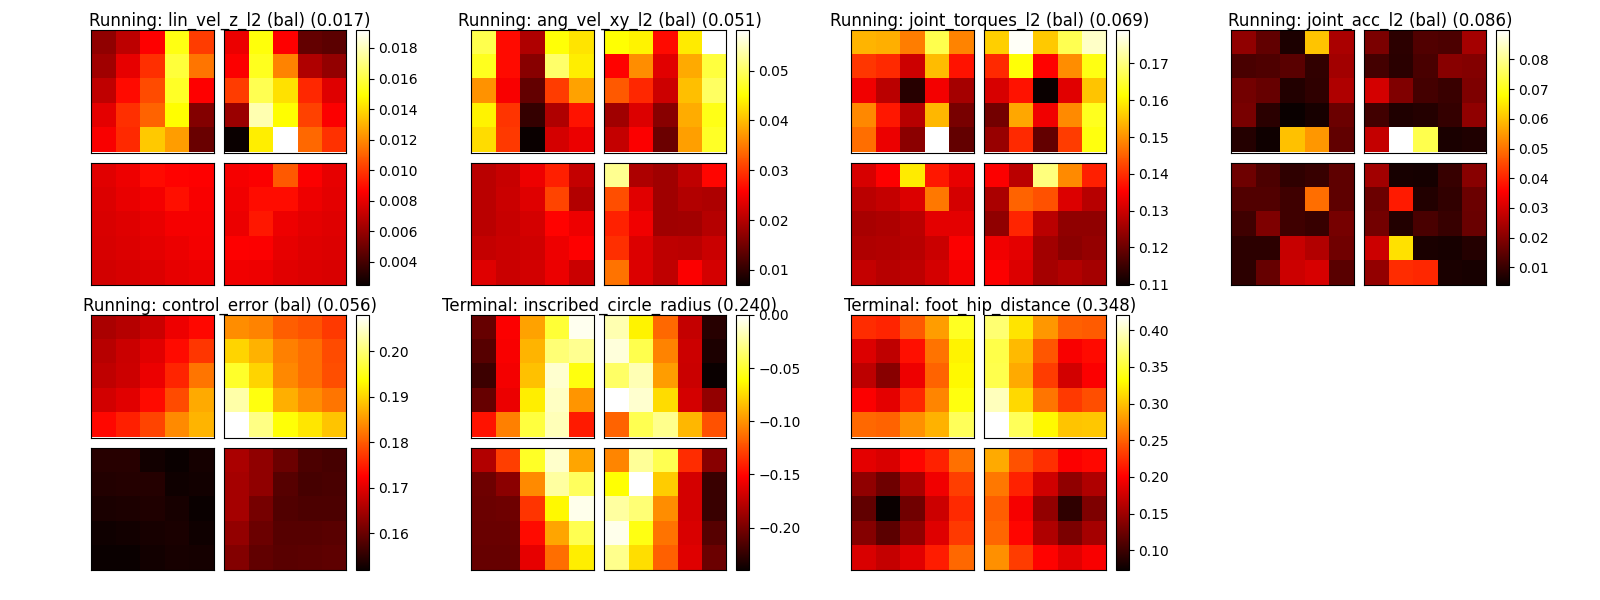
\includegraphics[width=\textwidth]{images/data/training/costmap-composition/elements.png}
    \caption{Factors influencing footstep cost maps. \textit{(bal)}
      indicates that the values for each leg were balanced to have a
      lower spread, mitigating factors that consistently prefer one leg
      over another. The last number in parenthesis indicates the total
    range of the data, the most important factor for the combined cost map.}
    \label{fig:data-costmap-composition-elements}
  \end{subfigure}
  \hfill
  \begin{subfigure}[T]{0.3\textwidth}
    \centering
    \includegraphics[width=\textwidth]{images/data/training/costmap-composition/combined.png}
    \caption{Combined cost map from factors in (a).}
    \label{fig:data-costmap-composition-combined}
  \end{subfigure}
  \hfill
\end{figure}

\begin{figure}
  \centering
  \includegraphics[width=0.5\textwidth]{images/data/training/training-fl-sweep.png}
  \caption{Snapshot showing 25 robots testing different footstep
    positions in parallel. For real data generation, 100 are run in
  parallel, testing 25 footstep positions for each foot at a time.}
\end{figure}

\begin{figure}
  \centering
  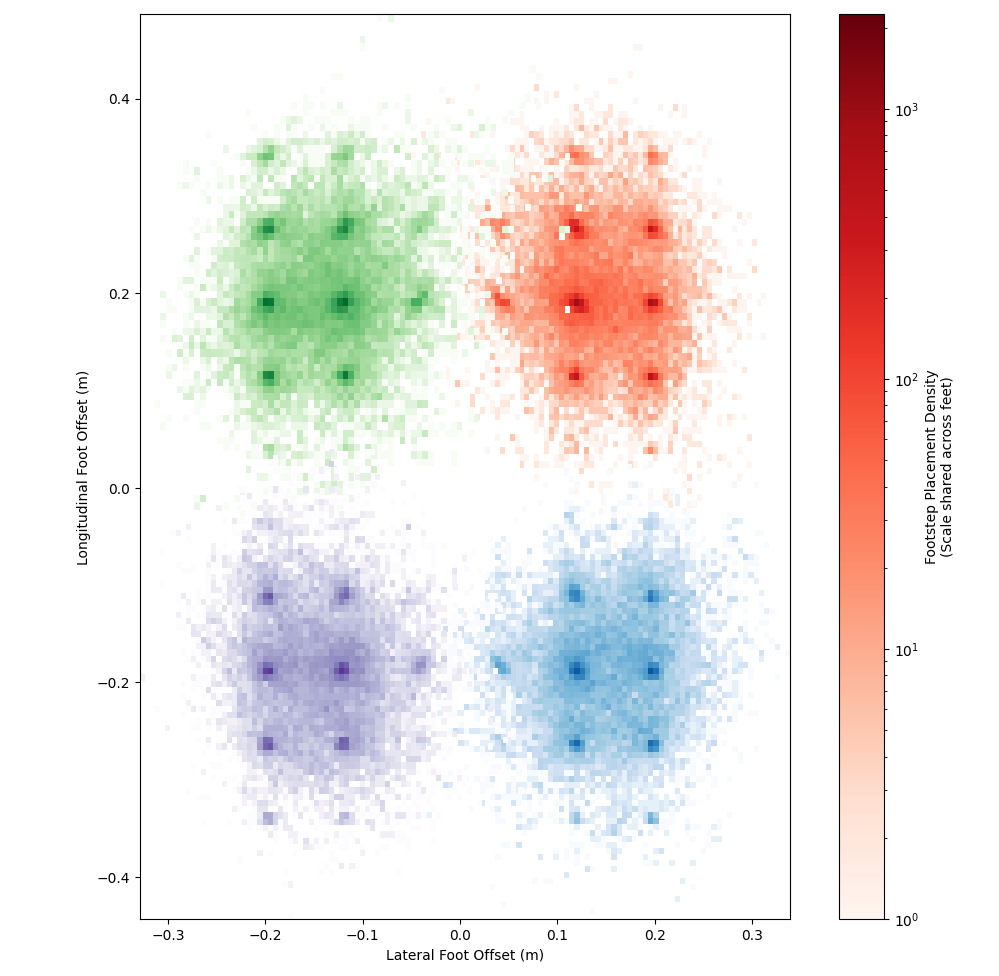
\includegraphics[width=0.5\textwidth]{images/data/foot-placement-heatmaps.png}
  \caption{Foot placement heatmaps showing distribution of foot
    positions in the GaitNet training data. Note that the histograms
  are overlaid in some places, obscuring data underneath.}
  \label{fig:data-cn-training-process}
\end{figure}

As in \cite{bratta_contactnet_2024}, the cost maps are normalized to
improve training performance. Our approach differs in how the cost
maps are normalized though. We directly normalize the cost maps to
the range $[0, 1]$, whereas \cite{bratta_contactnet_2024} normalizes
to $[0,1]$ in such a way that only the relative ordering of costs are
preserved. This difference is critical to our system to provide the
upstream GaitNet model with as much information as possible.

Below is the equation used as the input to the contact model.

\[
  \mathbf{x} =
  \begin{bmatrix}
    \mathbf p_{b,xy} \\
    \mathbf r_{w,z} \\
    \mathbf v_b \\
    \mathbf \omega_b \\
    \mathbf u
  \end{bmatrix}
\]

where
$\mathbf p_{b,xy}$ is the $x$ and $y$ position all end effectors in
the base frame stacked into a single vector,
$\mathbf r_{w,z}$ is the height of the robot's COM in the world frame.

The model is trained on $y$, the heuristically calculated footstep
cost maps (\autoref{fig:data-footstep-cost-map}).

\begin{figure}
  \centering
  \includegraphics[width=0.5\linewidth]{images/data/footstep-cost-map.png}
  \caption{Footstep cost map. Shows the heuristic cost for each
  possible footstep location.}
  \label{fig:data-footstep-cost-map}
\end{figure}

Here, the inclusion of $\mathbf \omega_b$ differs from
\cite{bratta_contactnet_2024}

%%%%%%%%%%%%%%%%%%%%%%%%%%%%%%%%%%%%%%%%%%%%%%%%%%%%%%%%%%%%%%%%%%%%%%%%%%%%%%%%
\subsection{Post-Processing}

Ultimately, the purpose of the footstep evaluation network is to
provide candidate footstep positions to the GaitNet model.
\autoref{fig:diagram-costmap-processing} shows the processing pipeline.
The raw cost map output (\autoref{fig:diagram-costmap-processing-raw})
from the footstep evaluation network is first upsampled
(\autoref{fig:diagram-costmap-processing-upsample}) to increase the
resolution of possible footstep positions, and to match the resolution of
the terrain data. Next, noise is added
(\autoref{fig:diagram-costmap-processing-noise}) to
encourage exploration of more varied footstep positions. Without noise,
all of the candidate footstep positions would be right next to each other.
The cost map is then filtered based on the robot state and terrain data
(\autoref{fig:diagram-costmap-processing-cspace}) to mask out
invalid actions, including positions that are too close to terrain edges,
and actions which would attempt to move a leg already in the swing state
(seen in the Front Right leg in this figure). Finally, the top 4
candidates from each leg are selected
(\autoref{fig:diagram-costmap-processing-topk})
to be processed by GaitNet.

% === Define layout constants ===
\def\imgwidth{0.16\textwidth}
\def\xgap{2em}          % horizontal gap between images
\def\arrowwidth{1.2em}  % controls arrow length
\def\arrowshift{0.5em} % vertical offset of arrows

\begin{figure}
  \centering
  \begin{tikzpicture}[node distance=\xgap, baseline=(current bounding
    box.center)]

    % === Style for image blocks ===
    \tikzset{
      imgblock/.style={inner sep=0pt, outer sep=0pt, align=center}
    }

    % === Subfigure nodes ===
    \node[imgblock] (a)
    {\subcaptionbox{Raw\label{fig:diagram-costmap-processing-raw}}%
    {\includegraphics[width=\imgwidth]{images/diagrams/cost-map-processing/1-default.png}}};

    \node[imgblock, right=of a]
    (b)
    {\subcaptionbox{Upsample\label{fig:diagram-costmap-processing-upsample}}%
    {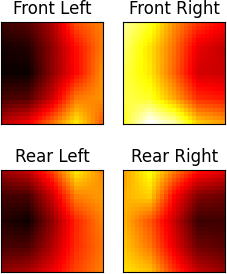
\includegraphics[width=\imgwidth]{images/diagrams/cost-map-processing/2-upscale.png}}};

    \node[imgblock, right=of b]
    (c)
    {\subcaptionbox{Noise\label{fig:diagram-costmap-processing-noise}}%
    {\includegraphics[width=\imgwidth]{images/diagrams/cost-map-processing/3-noise.png}}};

    \node[imgblock, right=of c]
    (d)
    {\subcaptionbox{C-space\label{fig:diagram-costmap-processing-cspace}}%
    {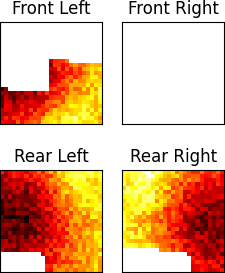
\includegraphics[width=\imgwidth]{images/diagrams/cost-map-processing/4-masked.png}}};

    \node[imgblock, right=of d]
    (e)
    {\subcaptionbox{TopK (green)\label{fig:diagram-costmap-processing-topk}}%
    {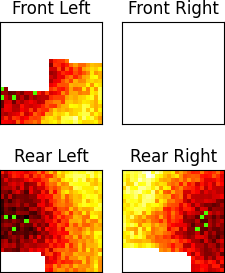
\includegraphics[width=\imgwidth]{images/diagrams/cost-map-processing/5-selected.png}}};

    % === Arrows ===
    \foreach \src/\dst in {a/b, b/c, c/d, d/e}{
      \draw[->, thick] ([yshift=\arrowshift]\src.east) --
      ++(\arrowwidth,0) --
      ([yshift=\arrowshift]\dst.west);
    }

  \end{tikzpicture}

  \caption{Cost map processing pipeline. Shows how the raw cost map
  is processed to produce the final footstep candidates.}
  \label{fig:diagram-costmap-processing}
\end{figure}
